\chapter{Evaluation}

This chapter will evaluate the effectiveness of the compiler developed in this project, by comparing
the generated LLVM IR code and the performance of the compiled code against other compilers
utilising the LLVM as a backend. A quantitative analysis will be discussed first, followed by an
analysis on the limitations of the compiler as implemented, and potential improvements that could be
made.

\section{Performance Benchmarking}

A key language feature ubiquitous in functional programming languages is the ability to define
recursive functions. A pure functional language paradigm will utilise recursion as a primary method
of iteration, as opposed to the traditional imperative loop constructs. Therefore, the ability for a
compiler to optimise recursive functions is crucial for the performance of the generated code.

The Ackermann function is a recursive computable function that grows rapidly with respect to its
inputs, and is a classic example used to benchmark the ability of a compiler to optimise recursive
calls.

The Ackermann function is defined as follows:

\singlespacing
\vspace{-0.7cm}
\begin{align*}
    ack(m, n) = \begin{cases}
        n + 1 & \text{if } m = 0 \\
        ack(m - 1, 1) & \text{if } m > 0 \text{ and } n = 0 \\
        ack(m - 1, ack(m, n - 1)) & \text{if } m > 0 \text{ and } n > 0
    \end{cases}
\end{align*}
\doublespacing

Despite the only arithmetic operation being an addition of one, even small inputs such as $ack(4,2)$
result in a value of $2 \times 10^{19728}$ due to the nested recursion, implying that the value of
the function is indicative of the running time of the function itself. Without proper optimisation,
the Ackermann function can quickly exhaust the call stack, and result in a stack overflow error. For
evaluation purposes, the Ackermann function will be evaluated for $m=3$ to restrict function growth
to (at most) exponential.

To properly evaluate the performance of the project compiler, the generated LLVM IR code was
compiled to a binary using the LLVM compiler (\texttt{llc}), and then linked against the C standard
library \texttt{libc} using the GNU Compiler Collection (\texttt{gcc}). Linking against
\texttt{libc} is necessary to provide the necessary \texttt{printf} function for output, as it not
defined in the LLVM. The resulting binary was then executed to measure the time taken to compute the
Ackermann function for various values of $n$.

The project compiler was benchmarked against Haskell (compiled with GHC), and C (compiled with
Clang). Haskell was chosen as a comparison due to its functional programming nature that has a
compiler compatible with the LLVM backend. C was chosen due to its high performance, and high
compatibility with the LLVM. (The LLVM was originally developed for C and C++ in
mind.~\autocite{lattner2004llvm})

Below is the implementation of the Ackermann function in all three languages:

\vspace{0.3cm}
\begin{tcbitemize}[raster columns=3, raster equal height=rows,size=small,space to upper]
    \tcbitem
        \footnotesize
        \begin{minted}{scala}
            def ack(m:Int, n:Int): Int =
                if m == 0 then
                    n+1
                else if n == 0 then
                    ack(m-1, 1)
                else
                    ack(m-1, ack(m, n-1));

            def main() = {
                print(ack(3,10))
                0
            }
        \end{minted}
        \tcblower
        \footnotesize $ack(m, n)$ in the project.
    \tcbitem
        \footnotesize
        \begin{minted}{haskell}
            ack :: Int -> Int -> Int
            ack 0 n = n+1
            ack m 0 = ack (m-1) 1
            ack m n = ack (m-1) (ack m (n-1))

            main = print (ack 3 10)
        \end{minted}
        \vfill
        \tcblower
        \footnotesize $ack(m, n)$ in Haskell.
    \tcbitem
        \scriptsize
        \begin{minted}{c}
            #include <stdio.h>

            int ack(int m, int n) {
                if (m == 0) {
                    return n+1;
                } else if (n == 0) {
                    return ack(m-1, 1);
                } else {
                    return ack(m-1, ack(m, n-1));
                }
            }

            int main() {
                printf("%d\n", ack(3, 10));
                return 0;
            }
        \end{minted}
        \tcblower
        \footnotesize $ack(m, n)$ in C.
\end{tcbitemize}
\vspace{0.4cm}

To ensure a fair comparison, and to evaluate the effect of the LLVM toolchain on compiler frontends,
all compilers were compiled at two optimisation levels: \texttt{-O0} and \texttt{-O3}. The
\texttt{-O0} flag disables all optimisations, while the \texttt{-O3} flag enables all
optimisations\footnote{The GHC compiler actually needs two optimisation flags to enable all; one for
GHC (\texttt{-O2}), and one for the LLVM (\texttt{-O3}).}. Each compiler was benchmarked ten times
with $ack(3,n)$ for each input value of $n$ (ranging from 10 to 15 inclusive) across both
optimisation levels, and the average time taken was recorded. The results of the benchmark are shown
in Table~\ref{tab:ackermann-benchmark}, and graphed in Figure~\ref{fig:ackermann-benchmark}.

\subsection{Results}

\begin{table*}\centering
    \renewcommand{\arraystretch}{1.3}
    \label{tab:ackermann-benchmark}
    \caption{Ackermann function benchmark results (in seconds)}

    \begin{tabular}{@{}lcccccccc@{}} \toprule
        Lang        & \multicolumn{2}{c}{Project} &              & \multicolumn{2}{c}{C} &              & \multicolumn{2}{c}{Haskell}                                  \\
        \cmidrule{2-3} \cmidrule{5-6} \cmidrule{8-9}
                    & \texttt{-O0}                & \texttt{-O3} &                       & \texttt{-O0} & \texttt{-O3}                &  & \texttt{-O0} & \texttt{-O3} \\ \midrule
        $ack(3,10)$ & 0.080                       & 0.024        &                       & 0.120        & 0.024                       &  & 1.334        & 0.101        \\
        $ack(3,11)$ & 0.312                       & 0.093        &                       & 0.490        & 0.092                       &  & 5.449        & 0.387        \\
        $ack(3,12)$ & 1.267                       & 0.370        &                       & 1.976        & 0.366                       &  & 22.63        & 1.578        \\
        $ack(3,13)$ & 5.071                       & 1.502        &                       & 8.088        & 1.495                       &  & 99.05        & 6.540        \\
        $ack(3,14)$ & 20.75                       & 6.193        &                       & 32.90        & 6.130                       &  & 475.3        & 28.08        \\
        $ack(3,15)$ & --                          & 24.74        &                       & --           & 23.26                       &  & 2237         & 127.1        \\
        \bottomrule
    \end{tabular}
\end{table*}

\begin{figure}
    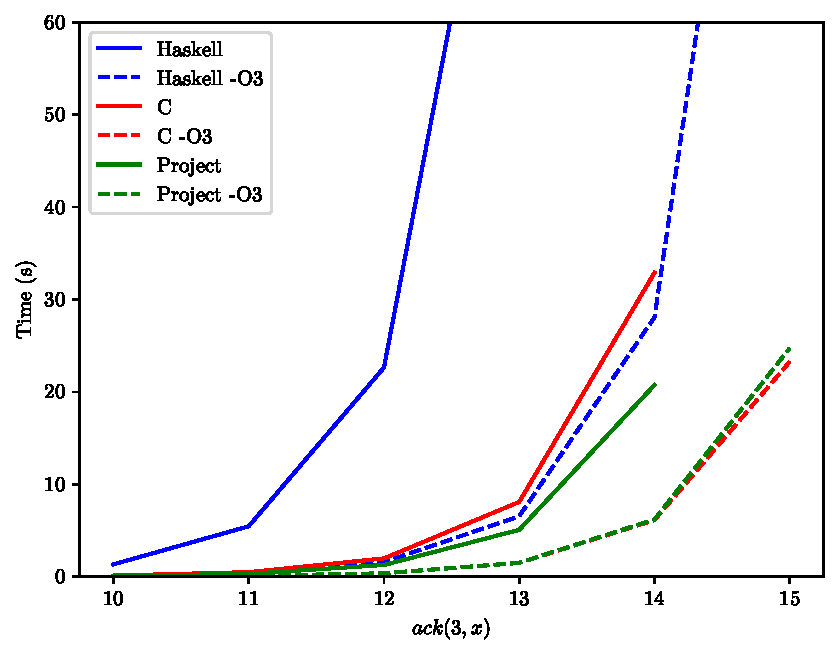
\includegraphics{Graphics/ackermann-benchmark.pdf}
    \caption{A graph reflecting the results of the Ackermann function benchmark.}
    \label{fig:ackermann-benchmark}
\end{figure}

The results show that, at optimisation level \texttt{-O0}, the
project compiler performs significantly better than Haskell, and slightly better than C across all
test cases.

On analysing the generated LLVM IR code, Clang (at \texttt{-O0}) appears copy all function arguments
to the stack as local variables before using them, occurring for each function invocation. This
results in many \texttt{alloca}, \texttt{store} and \texttt{load} instructions being called per
function call. The project compiler, on the other hand, utilises the LLVM's SSA form to eliminate
unnecessary memory operations, and instead uses the function arguments directly. This results in
significantly fewer memory related instructions, and a more efficient program.

A common behaviour observed in both the project compiler and Clang is the failure to compute the
Ackermann function for $ack(3,15)$, terminating with a segmentation fault. This is due to the
Ackermann function rapidly exhausting the call stack from the nested recursion. The project compiler
does not have an implementation for tail call optimisation, and Clang does not enable it by default.

On the other hand, the Haskell compiler is able to compute the function for $ack(3,15)$ without any
optimisations. This is likely due to Haskell lazy evaluation strategy, as it does not create stack
frames on each function call, but when an unevaluated value (a `thunk') is evaluated.

At optimisation level \texttt{-O3}, all compilers expectedly perform better than at \texttt{-O0},
but at different rates. The project compiler sees approximately a 3.3x improvement in performance, C
sees a 5x improvement, and Haskell sees a 14x improvement. The project compiler now performs almost
identically with C for small inputs, slightly dropping off as $n$ increases. Haskell, however, still
performs significantly worse than the other two compilers.

The generated LLVM IR code for the project compiler and Clang are now very similar, with both
utilising tail call optimisation to reduce the number of recursive calls inside the Ackermann
function down to one. This results in a significant reduction in the number of stack frames
required, and allows the function to be computed for larger inputs, such as $ack(3,15)$. This also
explains the very similar performance of the two compilers at \texttt{-O3}, as both compilers are
able to leverage the LLVM's optimisation passes to generate efficient code.

The primitive nature of the project compiler compared to other well-established compilers
notwithstanding, the results of the benchmark show that by leaning on the LLVM toolchain to perform
optimisations, the project compiler is able to generate efficient code that is in-line with other
compilers utilising the LLVM as a backend.

\section{Software Testing}

To ensure the correctness of the compiler, a suite of unit tests were written to test the various
phases of the compiler. The unit tests were written using the ScalaTest framework which test the
parser, enum refactor, IR generator, and closure conversion steps. The tests were written to cover a
range of scenarios, including edge cases. Where appropriate, mock objects were used to isolate the
unit under test from its dependencies (e.g. the generation of unique variable names).

Provided are example unit tests for the enum refactor stage:

\begin{code}{scala}
class EnumSpec extends AnyFlatSpec {
    // ... other tests ...

    behavior of "Match to If transformation"

    it should "correctly transform a match statement with a default case" in {
        val m = Match("a", List(MCase("A", "B", Num(6)), MCase("", "_", Num(5))))
        val expected = If(Op(Var("a"), "==", EnumRef("A", "B")), Num(6), Some(Num(5)))
        assert(transform_match_to_if(m) == expected)
    }

    it should "correctly transform a match statement with multiple cases" in {
        val m = Match("a", List(MCase("A", "B", Num(6)), MCase("C", "D", Num(5))))
        val expected = If(Op(Var("a"), "==", EnumRef("A", "B")), Num(6), Some(If(Op(Var("a"), "==", EnumRef("C", "D")), Num(5), Some(Op(Num(0), "+", Num(0))))))
        assert(transform_match_to_if(m) == expected)
    }

    it should "correctly transform a match statement with multiple cases and a default case" in {
        val m = Match("a", List(MCase("A", "B", Num(6)), MCase("C", "D", Num(5)), MCase("", "_", Num(4))))
        val expected = If(Op(Var("a"), "==", EnumRef("A", "B")), Num(6), Some(If(Op(Var("a"), "==", EnumRef("C", "D")), Num(5), Some(Num(4)))))
        assert(transform_match_to_if(m) == expected)
    }

    it should "correctly skip other cases after a default case" in {
        val m = Match("a", List(MCase("A", "B", Num(6)), MCase("", "_", Num(5)), MCase("C", "D", Num(4))))
        val expected = If(Op(Var("a"), "==", EnumRef("A", "B")), Num(6), Some(Num(5)))
        assert(transform_match_to_if(m) == expected)
    }
}
\end{code}

As seen, the tests are written in a BDD (Behaviour-driven development) style, with each test case
describing the expected behaviour of the function under test. In total, 50 unit tests were written
to test the various phases of the compiler.

% TODO tests

\section{Limitations}

It is near impossible to claim any compiler is perfectly implemented against the specification of a
language. This project is no exception, and has a number of limitations that prevent it from being
considered a complete compiler. The following sections will discuss some limitations of the project
compiler, and potential improvements that could be made.

\subsection{Heap-allocated variables}

The project compiler does not support heap-allocated variables. All variables are stack-allocated,
and are deallocated when they go out of scope. This can be problematic for programs that require
variables to persist beyond the scope in which they were defined, such as returning a struct from a
function. Additionally, the implementation of data structures based on lists (e.g. Strings) is
limited without heap-allocated variables.

Adding support for heap-allocated variables would require a refactor of the code generation phase.
The code generation phase would need to be modified to allocate memory on the heap for variables
that need to persist beyond the scope in which they were defined, and to deallocate memory when the
variables are no longer needed. Without providing explicit functions for memory management to the
end-user, this would typically be implemented in the form of a garbage collector.

\subsection{Recursive Structures}

The project compiler does not support recursive structures. This can be problematic for programs
that require recursive data structures, such as linked lists or trees. The lack of support for
recursive structures can make it difficult to write programs that manipulate complex data
structures.

Adding support for recursive structures would require a significant refactor of the code generation
phase. The code generation phase would need to be modified to allocate memory on the heap for
recursive structures, and to generate code that correctly traverses and manipulates the structures.

\subsection{Sum Types}

The project compiler does not support sum types. Sum types are a common feature of functional
programming languages, and are used to represent a value that can take on one of several different
forms. The lack of support for sum types can make it difficult to write programs that manipulate
complex data structures.

Adding support for sum types would require a significant refactor of the code generation phase. The
code generation phase would need to be modified to allocate memory on the heap for sum types, and to
generate code that correctly handles the different forms of the types.

\subsection{Error Handling}

The project compiler has very limited error handling capabilities. The parser is able to detect
syntax errors, and the type checker is able to detect type errors, but the error messages are not
very informative, and do not provide much context to the user. The error messages are also not
localised, and do not provide the location of the error in the source code.

Improving the error handling capabilities of the compiler would require a significant refactor of the
parser and type checker phases. The parser would need to be modified to provide more informative
error messages, and the type checker would need to be modified to provide more context to the user.

\subsection{Code Generation}

The code generation phase of the project compiler is very basic, and does not perform any
optimisations. The generated LLVM IR code is very verbose, and contains a lot of redundant
instructions. This can result in inefficient code that is difficult to read and understand. The
project compiler also does not generate any debug information, which can make it difficult to
debug the generated code.

Improving the code generation capabilities of the compiler would require a significant refactor of
the code generation phase. The code generation phase would need to be modified to perform
optimisations such as constant folding, dead code elimination, and common subexpression elimination.
The code generation phase would also need to be modified to generate debug information, such as line
numbers and variable names.



